\noindent A segunda função escolhida foi \(f_2(x) = x^3 - 2\). O código implementado para construção do gráfico e da tabela é semelhante ao da função anterior:

\lstinputlisting{II/f2.m}
O gráfico e a tabela obtidos são os seguintes:

\begin{figure}[ht]
    \centering
    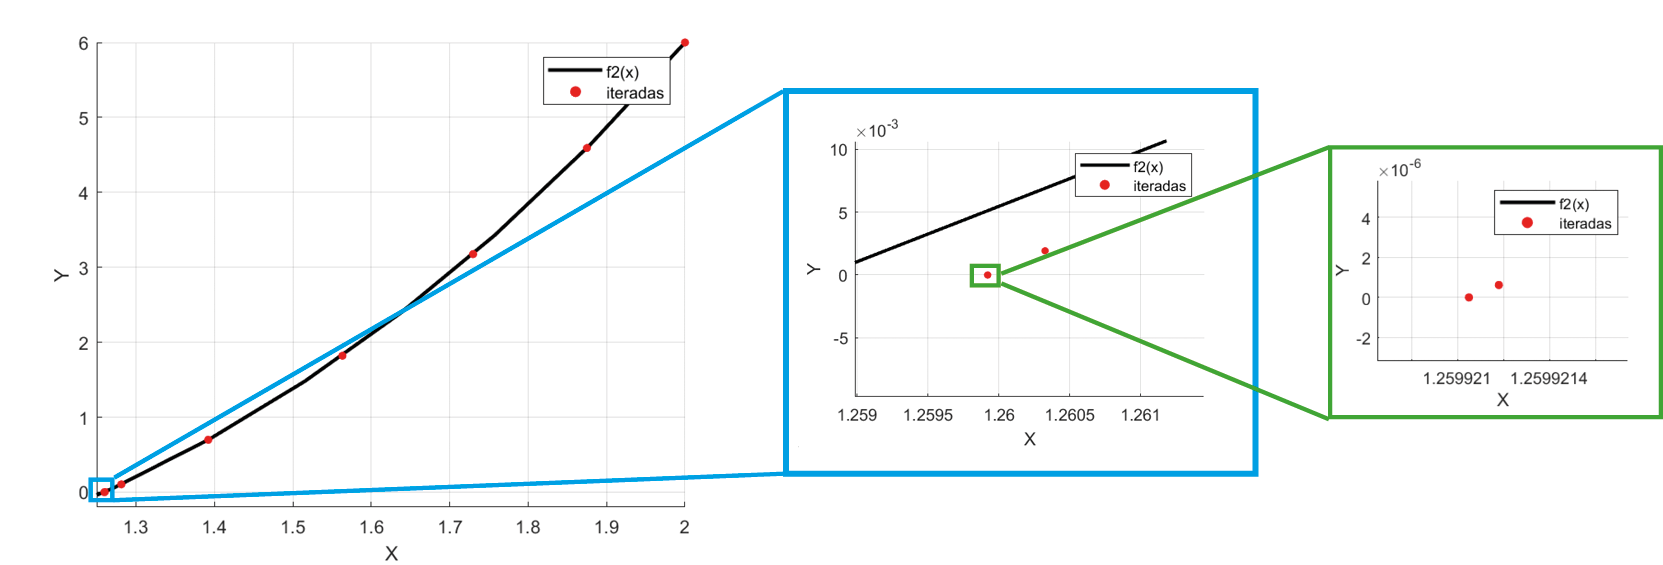
\includegraphics[width=\textwidth]{II/grafico_f2.png}
    \label{grafico_f2}
\end{figure}

\begin{table}[ht]
    \centering
    \begin{tabular}{|c|c|c|c|c|c|}
    \hline
    \(n\) & \(x_n\) & \(|e_n|\) & \(\displaystyle \frac{|e_{n+1}|}{|e_n|}\) & \(\displaystyle \frac{|e_{n+1}|}{|e_n|^2}\) & \(\displaystyle \frac{|e_{n+1}|}{|e_n|^3}\) \\
    \hline
    0 & $2.000000000000000$ & $0.740078$                & $0.831099$               & $1.122987$ & $1.51738$ \\
    1 & $1.875000000000000$ & $0.615078$                & $0.763988$               & $1.242098$ & $2.01941$ \\
    2 & $1.729834556821689$ & $0.469913$                & $0.645474$               & $1.373602$ & $2.92309$ \\
    3 & $1.563238177806971$ & $0.303317$                & $0.436235$               & $1.438215$ & $4.74162$ \\
    4 & $1.392238676508353$ & $0.132317$                & $0.162335$               & $1.226863$ & $9.27210$ \\
    5 & $1.281400912585896$ & $0.021479$                & $0.018825$               & $0.876420$ & $40.8019$ \\
    6 & $1.260325416620598$ & $4.043667 \times 10^{-4}$ & $3.21587 \times 10^{-4}$ & $0.795285$ & $1.96674 \times 10^3$ \\
    7 & $1.259921179934046$ & $1.300391 \times 10^{-7}$ & & & \\
    8 & $1.259921049894887$ & & & & \\
    \hline
    \multicolumn{6}{|c|}{$p = 2\quad K_{\infty} \approx 0.8$}\\
    \hline
    \end{tabular}
\end{table}

\noindent Pelo gráfico percebe-se que, de facto, as iteradas estão a convergir para \(z\). Os valores da tabela permitem concluir que \(\displaystyle \frac{|e_{n+1}|}{|e_n|}\) deve convergir para 0 e \(\displaystyle \frac{|e_{n+1}|}{|e_n|^3}\) deve convergir para \(\infty\). Já os valores \(\displaystyle \frac{|e_{n+1}|}{|e_n|^2}\) devem convergir para um \(K_\infty \approx 0.8\), mostrando a convergência de ordem 2.